%
% curve.tex -- Brechung an einem Kreis
%
% (c) 2018 Prof Dr Andreas Müller, Hochschule Rapperswil
%
\documentclass[tikz,12pt]{standalone}
\usepackage{times}
\usepackage{amsmath}
\usepackage{txfonts}
\usepackage[utf8]{inputenc}
\usepackage{graphics}
\usepackage{color}
\usepackage{pifont}
\usetikzlibrary{arrows,intersections,math,calc}
\begin{document}

\def\punkt#1{
        \fill[color=white] #1 circle[radius=0.08];
        \draw #1 circle[radius=0.08];
}

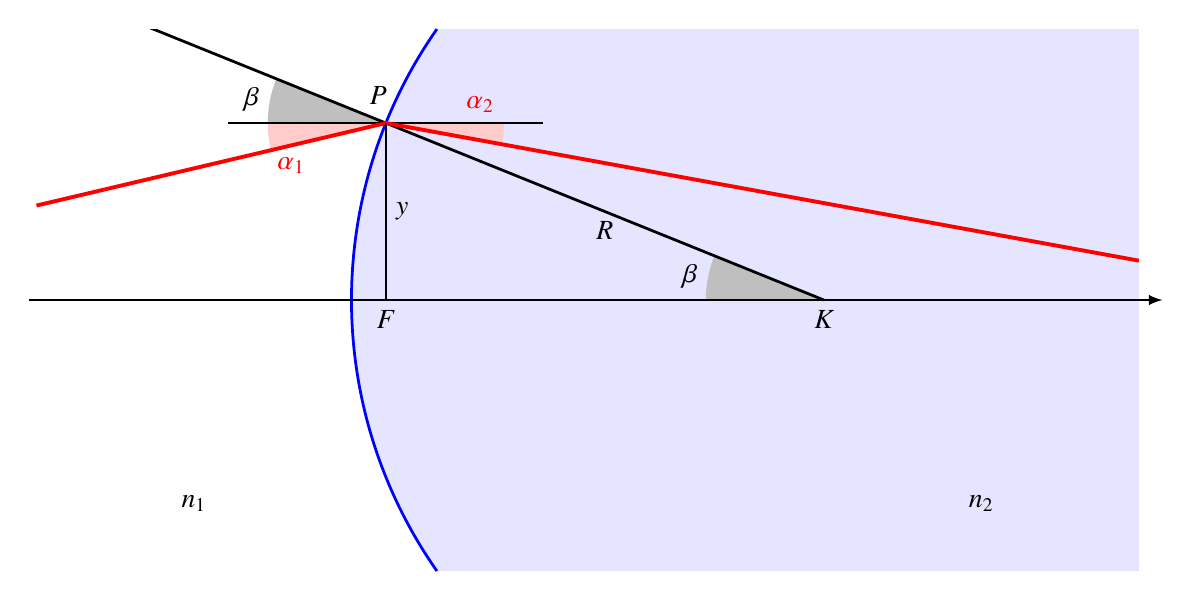
\begin{tikzpicture}[>=latex,thick]

\def\R{6}
\def\a{35}
\def\b{22}
\def\w{4}

\pgfmathparse{\R*sin(\a)}
\xdef\h{\pgfmathresult}

% Linse
\fill[color=blue!10] ({\w},{\h})
	--
	({-\R*cos(\a)},{\R*sin(\a)}) arc (180-\a:180+\a:\R)
	--
	({\w},{-\h})--cycle;
\draw[color=blue,line width=1pt]
	({-\R*cos(\a)},{\R*sin(\a)}) arc (180-\a:180+\a:\R);

% Winkel bei K
\fill[color=gray!50] (0,0)
	--
	({-1.5*cos(\b)},{1.5*sin(\b)}) arc ({180-\b}:180:1.5)
	--cycle;
\fill[color=gray!50]
	({-\R*cos(\b)},{\R*sin(\b)})
	--
	({-(\R+1.5)*cos(\b)},{(\R+1.5)*sin(\b)}) arc ({180-\b}:180:1.5)
	--cycle;
\node at ({-\R*cos(\b)-1.7},{\R*sin(\b)+0.3}) {$\beta$};
\node at ({-1.7},{+0.3}) {$\beta$};

\fill[color=red!20]
	({-\R*cos(\b)},{\R*sin(\b)})
	--
	({-\R*cos(\b)+1.5},{\R*sin(\b)}) arc (0:-10:1.5)
	--cycle;
\node[color=red] at ({-\R*cos(\b)+1.2},{\R*sin(\b)}) [above] {$\alpha_2$};
\fill[color=red!20]
	({-\R*cos(\b)},{\R*sin(\b)})
	--
	({-\R*cos(\b)-1.5},{\R*sin(\b)}) arc (180:193:1.5)
	--cycle;
\node[color=red] at ({-\R*cos(\b)-1.2},{\R*sin(\b)-0.3}) [below] {$\alpha_1$};

% Radius
\begin{scope}
\clip (-10,{-\h}) rectangle ({\w},{\h});

\draw[line width=1.0pt] (0,0)--({-10*cos(\b)},{10*sin(\b)});

\end{scope}

\node at ({-\R*cos(\b)-0.1},{\R*sin(\b)+0.1}) [above] {$P$};
\draw[line width=0.5pt]
({-\R*cos(\b)-2},{\R*sin(\b)})
--
({-\R*cos(\b)+2},{\R*sin(\b)});

% Strahl
\draw[color=red,line width=1.4pt] (-10,1.2)
	--
	({-\R*cos(\b)},{\R*sin(\b)})
	--
	(4,0.5);

% y
\draw[line width=0.5pt]
	({-\R*cos(\b)},0)--
	({-\R*cos(\b)},{\R*sin(\b)});
\node at ({-\R*cos(\b)},{\R*sin(\b)/2}) [right] {$y$};

% optische Achse
\draw[->,line width=0.7pt] (-10.1,0)--({\w+0.3},0);

\punkt{(0,0)}
\punkt{({-\R*cos(\b)},{\R*sin(\b)})}
\node at (0,0) [below] {$K$};

\node at ({-\R*cos(\b)/2},{\R*sin(\b)/2}) [below] {$R$};

\node at ({-\R*cos(\b)},0) [below] {$F$};
\punkt{({-\R*cos(\b)},0)}

\node at (-8,{-3*\h/4}) {$n_1$};
\node at ({\w-2},{-3*\h/4}) {$n_2$};


\end{tikzpicture}

\end{document}

